\chapter{The Lifecycle of Deep Convective Cores and their Associated Anvil Clouds Observed over North America}


% \begin{abstract}
% Deep convective clouds play an important role in the climate and are the cause of a number of extreme weather events.
% As global warming causes an increase in the frequency of storms and related extreme weather events, it is vital that we better understand the response of deep convective clouds to anthropogenic influences.
% Observing these impacts is, however, difficult due to both the complex behaviour of these clouds and the many interactions and feedbacks between deep convective clouds and the environment.

% By developing a novel method for detecting deep convective clouds, we can detect and track cores and their associated anvil clouds over their entire lifetime.
% Using a year of observations over the continental United States, we analyse the properties of developing deep convective cores and anvil clouds, and how these properties are linked.
% The spatial patterns of observed convection show notable changes with the seasonal cycle.
% Furthermore, we observe differences in the diurnal distribution of deep convection between different regions, and impacts of the diurnal cycle on the properties of observed developing deep convective clouds.
% In particular, we see strong land/sea contrast, the impact of the sea-breeze effect on convective initiation in coastal regions, and an increase in the intensity of convective growth with later time of initiation over the Great Plains region.
% Despite these changes, some properties -- such as the lifetime of the developing cloud core -- show little regional variation.
% Finally, we link the properties of growing cores to those of single- and multi-core anvils, and show how multi-core anvils can have larger lifetimes and extents, despite the properties of individual cores being similar to those of single-core anvils.

% \end{abstract}




\section{Introduction}  %% \introduction[modified heading if necessary]



\section{Data}

To detect and track \acrshort{dcc}s across North America, we use \acrshort{abi} \acrshort{mcmip} data from the 6.2, 7.3, 10.4 and 12.4\,\unit{\mu m} channels observed in the \acrshort{conus} region, as described in section \ref{sec:abi_data}.
We use the full extent of the \acrshort{abi} \acrshort{conus} domain of 2,500~pixels E--W by 1,500~pixels N--S.
This domain covers a region of around 60--120\,\textdegree W in longitude and 15--60\,\textdegree N in latitude, covering an area of approximately 5,700 by 3,900\,\unit{km}.
Figure~\ref{fig:abi_zenith_angles} shows the satellite zenith angle of \acrshort{abi} observations across the \acrshort{conus} domain.
The large sensor zenith angles in the North-West of the domain may introduce large errors in the detection and tracking algorithm, so for the rest of this chapter we will only consider \acrshort{dcc}s detected east of 120\,\textdegree W and south of 50\,\textdegree N.
As the viewing angle increases detection and tracking become more difficult.
This is due to the confounding between vertical and horizontal motion, and also due to the area of each pixel increasing with the zenith angle.

\begin{figure}[tp]
    \centering
    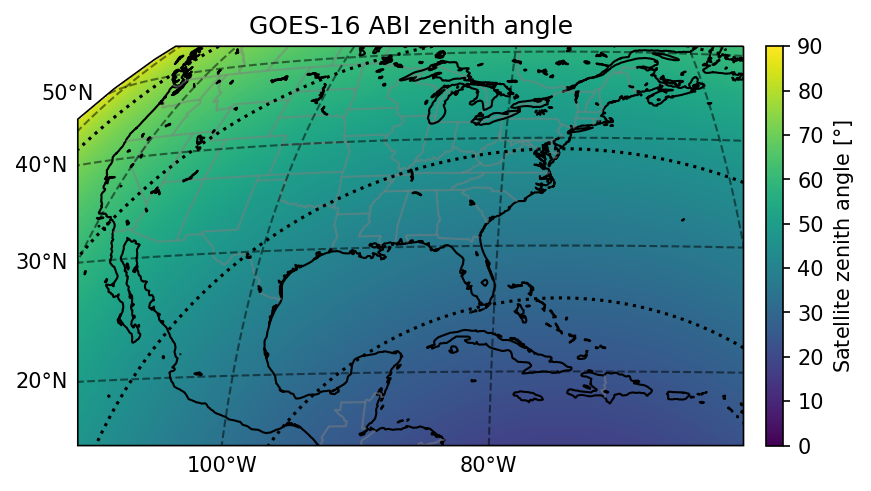
\includegraphics[width=\textwidth]{figures/ch2_01.png}
    \caption[
    The sensor zenith angle of \acrshort{goes}-16 \acrshort{abi} observations across the \acrshort{conus} domain
    ]{
    The sensor zenith angle of \acrshort{goes}-16 \acrshort{abi} observations across the \acrshort{conus} domain. Dotted arcs are shown for each 15\,\textdegree interval of zenith angle. Zenith angles in the north-west corner of the domain are particularly large, and so any observed \acrshort{dcc}s further north than 50\,\textdegree N or west of 120\,\textdegree W are removed from subsequent analysis.
    }
    \label{fig:abi_zenith_angles}
\end{figure}

Five full years of data---from the start of 2018 to the end of 2022---are used to produce a dataset of detected \acrshort{dcc}s and their properties.
This period spans all complete years of operational data from \acrshort{goes}-16 \acrshort{abi}.
To improve to continuity of observations, we then perform a gap-filling procedure.
If time gaps between observations of greater than 15 minutes are present we use observations from the full-disc \acrshort{abi} scan to fill these gaps.
Full disc imagery is typically available every 10 or 15 minutes depending on the operating mode.
This gap filling is particularly important during the periods in which \acrshort{abi} uses its mode 4 scan pattern, in which no \acrshort{conus} domain scans are made, but the full-disc is scanned every 5 minutes.
Using the full-disc observations allows us to maintain temporal sampling throughout these periods.


\section{Method}

Detection and tracking of convective cores and anvil cloud is performed using the method described in section~\ref{sec:tracking_method}.
Initial detection of \acrshort{dcc}s is performed separately over 24-hour periods spanning from 12:00:00~\acrshort{utc} (approximately 6am local time over North America) to the same time the next day.
This 24-hour period was dictated due to performance constraints, as the large domain combined with the high spatial and temporal resolution of \acrshort{abi} data results in a large memory requirement.
This time corresponds with the minima of convective activity over land, and so was chosen in order to minimise the number of \acrshort{dcc}s missed at the start and end of the detection period.
Each period is extended by six \acrshort{abi} observations at each end to ensure at least one hour of overlap between successive days.

To track long-lived \acrshort{dcc}s that last beyond one day, we apply a linking algorithm which combines \acrshort{dcc}s observed across multiple days.
The linking algorithm combines \acrshort{dcc}s detected at the same locations within the overlap period of two daily detection files.
Splitting and merging of objects is taken into account, so a single object which splits into two, or two objects which merge into one in the subsequent file are all considered a single, tracked object.
The linking algorithm is applied separately to each month of data for performance reasons.

After linking, a processing step is applied to calculate the properties of detected cores and anvils at each step of their lifecycles.
Finally, core and anvil step properties are aggregated over each month of observation, and overall core and anvil properties are calculated.
During this final step quality flagging is performed to isolate detected features that fail one or more quality checks.
The quality criteria are split into two criteria.
The first set of criteria---for core or anvil removal---removes detected features which should not pass the criteria for detection in the first place.
Detected features which flag any of these criteria are removed from the aggregated dataset in their entirety.
This step in particular removes anvils which have no cores associated with them, or are not detected as initiating with a developing core.

The second set of criteria is used to identify detected cores or anvils for which we do not observe their entire extent or lifecycle.
Cores and anvils which flag are of these criteria are still included within the aggregated properties dataset, but are not used when investigating \acrshort{dcc} properties throughout this chapter.

Quality criteria for cores are listed in table \ref{table:core_validity_criteria}, and those for anvils in tabel \ref{table:anvil_validity_criteria}.

%t
\begin{table}[tb]
\centering
\begin{tabular}{ll}
\tophline
Core removed if:                                                    & Core invalid if: \\
\middlehline
Initial \acrshort{bt} -- final \acrshort{bt} \textless~8\,\unit{K}  & Intersects edge of domain \\
Lifetime \textless~15~minutes                                       & Intersects start of domain \\
Time gaps \textgreater~15~minutes                                   & Intersects end of domain \\
Maximum area \textgreater~10,000\,\unit{km\textsuperscript{2}}      & Adjacent to bad \acrshort{abi} data \\
Any NaN values in core properties                                   & \\
\bottomhline
\end{tabular}
\caption[
Validity criteria for detected cores
]{
Validity criteria for detected cores. Cores which flag any of the removal criteria are removed in their entirety from the dataset. Those which flag any of the invalid criteria are retained, but removed from subsequent analysis.}
\label{table:core_validity_criteria}
\end{table}


%t
\begin{table}[tb]
\centering
\begin{tabular}{ll}
\tophline
Anvil removed if:                               & Anvil invalid if: \\
\middlehline
No associated cores                             & Intersects edge of domain \\
Lifetime \textless~15~minutes                   & Intersects start of domain \\             
Time gaps \textgreater~15~minutes               & Intersects end of domain \\
Maximum area \textless~maximum core area        & Adjacent to bad \acrshort{abi} data \\
Anvil detected before initial core              & Associated with invalid cores \\
Anvil dissipated before final core ends         & Maximum area reached before end \\
Any NaN values in anvil properties              & ~~of initial core \\
\bottomhline
\end{tabular}
\caption[
Validity criteria for detected anvils
]{
Validity criteria for detected anvil. Anvils which flag any of the removal criteria are removed in their entirety from the dataset. Those which flag any of the invalid criteria are retained, but removed from subsequent analysis. The majority of anvils removed are due to have no associated cores, or because the anvil was observed before any developing cores.}
\label{table:anvil_validity_criteria}
\end{table}


The complete processing pathway is outlined by the following steps:

\begin{enumerate}
    \item Detection of cores and anvils in \acrshort{abi} observations over each 24-hour period.
    \item Linking of overlapping objects detected in subsequent 24-hour periods over each month.
    \item Calculation of core and anvil step properties. 
    \item Quality criteria applied to core and anvils, properties aggregated over each month
\end{enumerate}

Two datasets are produced. The first consists of daily core and anvil spatial maps, with step properties, produced by processing step 3. 
The second, consisting of aggregated monthly core and anvil properties, is produced by step 4.

Figure~\ref{fig:conus_detected_dccs} shows an example of detected cores and anvils over the \acrshort{conus} region, against backgrounds of composite visible imagery (fig.~\ref{fig:conus_detected_dccs}\,a) and 10.4\,\unit{\mu m} \acrshort{bt} (fig.~\ref{fig:conus_detected_dccs}\,b).
Cores and anvils which are removed from the aggregated dataset are outlined with dotted lines, and those which are marker invalid are shown with dashed outlines.

\begin{figure}[tp]
    \centering
    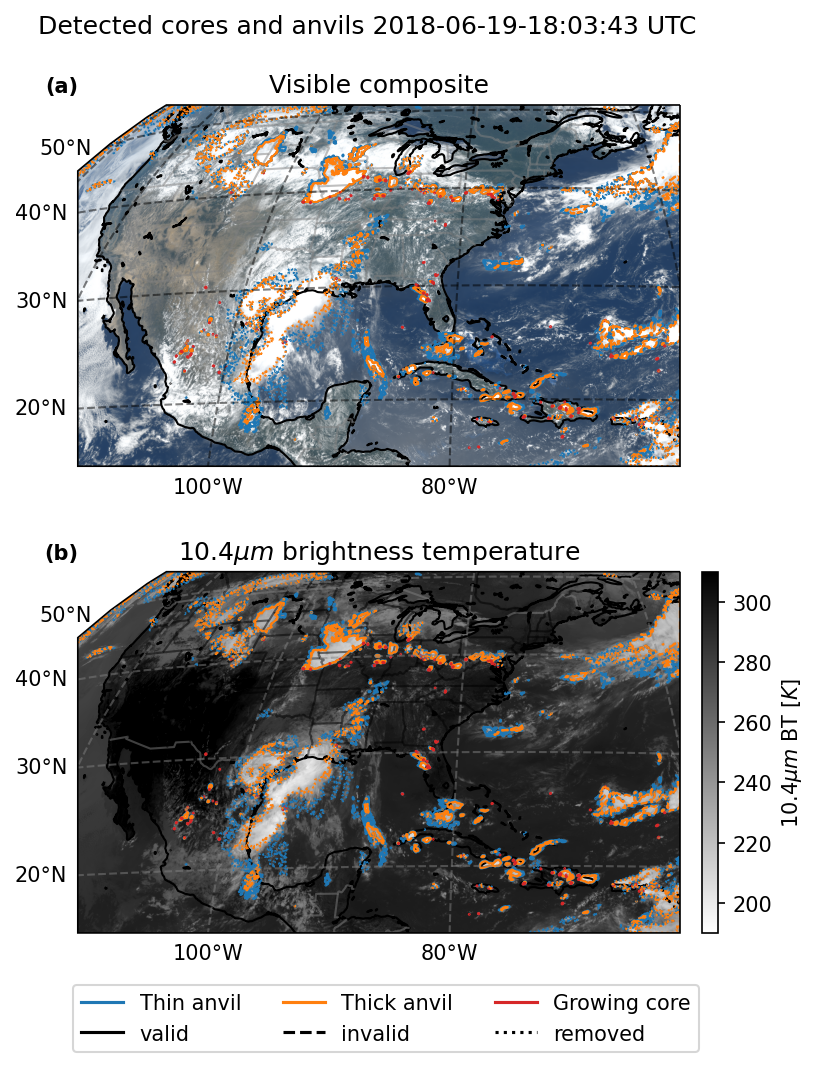
\includegraphics[width=\textwidth]{figures/ch2_02.png}
    \caption[
    Detected cores and anvils from a snapshot of \acrshort{goes}-16 \acrshort{conus} domain observations
    ]{
    Detected cores and anvils from a snapshot of \acrshort{goes}-16 \acrshort{conus} domain observations. Cores and anvils removed from the aggregated dataset are shown with dotted outlines. Those which are flagged as invalid are shown with dashed outlines. Detected features are shown against (a) visible composite imagery and (b) 10.4\,\unit{\mu m} \acrshort{bt}
    }
    \label{fig:conus_detected_dccs}
\end{figure}

Over the five-year observing period we detect a total of 3,877,130 cores, of which 3,817,286 are valid, and 648,345 anvils, of which 576,555 are valid.

\section{Results}

% \section{A novel method for detecting deep convective cloud cores and their associated anvils in geostationary satellite imagery}

% Numerous algorithms have been developed for the purpose of automatically detecting and tracking \acrshort{dcc}s, and are widely used for both forecasting and research purposes \citep[e.g.][]{mecikalski_use_2011, senf_characterization_2015, senf_satellite-based_2017, feng_life_2012, feng_spatiotemporal_2019, zinner_cb-tram:_2008}.
% Development of these algorithms has seen constant and continuous efforts.
% However a number of difficulties must be taken into account when utilising geostationary satellite imagery to detect and track \acrshort{dcc}s compared to the use of radar or lightning observations.

%f
% \begin{figure*}[t]
%     \centering
%     \includegraphics[width=12cm]{figure01.pdf}
%     \caption{Observations of a cluster of deep convective clouds over North-West Florida throughout three stages of their lifecycle. This cluster of \acrshort{dcc}s occurred on the afternoon of 19\textsuperscript{th} June 2018. The "growing" column were observed at 17:00 UTC, the "mature" column at 19:00 UTC, and the dissipating column at 21:00 UTC. Note that, unless otherwise specified, this case study is used for all subsequent figures in this article.}
%     \label{fig:compare_sat_radar_glm}
% \end{figure*}

% Figure \ref{fig:compare_sat_radar_glm} provides an example of how geostationary satellite imagery compares to observations of \acrshort{dcc}s using ground-based cloud radar and lightning observations.
% In fig. \ref{fig:compare_sat_radar_glm}a, \ref{fig:compare_sat_radar_glm}d, \ref{fig:compare_sat_radar_glm}g and \ref{fig:compare_sat_radar_glm}e, we see how a growing \acrshort{dcc} is observed by visible/near infrared (NIR) satellite imagery, 10.4\,\unit{\mu m} longwave (LW) infrared (IR) satellite imagery, lightning flash observations from a satellite instrument and column radar reflectivity respectively.
% Figures \ref{fig:compare_sat_radar_glm}b, \ref{fig:compare_sat_radar_glm}e, \ref{fig:compare_sat_radar_glm}h and \ref{fig:compare_sat_radar_glm}k show observations of a mature \acrshort{dcc}, and \ref{fig:compare_sat_radar_glm}c, \ref{fig:compare_sat_radar_glm}f, \ref{fig:compare_sat_radar_glm}i and \ref{fig:compare_sat_radar_glm}l show those of a dissipating \acrshort{dcc}.
% While lightning and radar observations are capable of detecting deep convection in the growing and mature phase of \acrshort{dcc}s, neither can detect either the full extent of the anvil cloud or the dissipating phase of the \acrshort{dcc}.
% The ability to detect and track the anvil cloud over its entire lifetime is important to study the anvil cloud radiative forcing on the climate, the response to temperature change \citep{bony_thermodynamic_2016, hartmann_tropical_2016, ceppi_cloud_2017, gasparini_what_2019} and possible feedbacks on subsequent convective activity \citep{varble_erroneous_2018}.
% However, while radar and lightning observations of \acrshort{dcc}s can directly detect deep convection due to the strong correlations between core updraft intensity and radar reflectivity and polarisation \citep{austin_relation_1987, rosenfeld_general_1993, zipser_vertical_1994},  and lightning flash occurrence \citep{williams_relationship_1989, deierling_total_2008, wang_relationship_2017}, the same is not possible for geostationary satellite observations.
% Instead, a proxy variable linked to convective activity must be used to detect \acrshort{dcc}s.

% There are, in general, two approaches used as proxies for detecting convective clouds in geostationary satellite imagery. 
% Firstly, thresholds on observed field -- in particular LW IR brightness temperature (BT) -- are capable of detecting \acrshort{dcc} anvil clouds \citep[e.g.][]{schmetz_monitoring_1997, hong_detection_2005, schroder_deep_2009, liang_integrated_2017, senf_size-resolved_2018}.
% Secondly, the early stages of \acrshort{dcc}s can be detected using cloud top cooling rates \citep{zinner_cb-tram:_2008, bedka_objective_2010, muller_novel_2019}.
% The latter method is typically used for early detection of \acrshort{dcc}s for forecasting systems, as cloud top growth can detect \acrshort{dcc}s prior to radar observations \citep{roberts_nowcasting_2003}.
% While such algorithms provide an accurate detection of these early phases of \acrshort{dcc} growth \citep{zinner_validation_2013}, as the cooling of the cloud top is only visible during the initial phase of the \acrshort{dcc} any method that solely relies on detecting the growth of the \acrshort{dcc} will be unable to detect the anvil cloud after this initial growth phase has ended.

% On the other hand, threshold-based methods are better capable of detecting \acrshort{dcc}s throughout the mature phase, however are less able to detect the early stages of \acrshort{dcc} growth due to the inability to distinguish warm, growing \acrshort{dcc}s from other warm clouds.
% Furthermore, the choice of threshold value presents a limitation to the accuracy of threshold based detection methods.
% A choice of a warmer BT threshold results in false detections of non-convective clouds, whereas a colder threshold results in missed detections of \acrshort{dcc}s which do not meet the threshold, and further reduces the period over which \acrshort{dcc}s are detected.
% As the distributions of cloud top temperature for \acrshort{dcc}s and non-convective clouds overlap \citep{so_classification_2018}, there is no ideal threshold value that avoids this issue.
% \citet{fiolleau_algorithm_2013} implemented a single-step framework for detecting and tracking MCSs that aims to address the compromise in detection accuracy by allowing a \acrshort{dcc} that is detected above a cold threshold BT at any time-step to be detected and tracked across the rest of its lifetime using a warmer threshold.
% Whereas this approach is successful for large, mesoscale systems, where the advection of the anvil is small compared to the over anvil area, it is less suitable for tracking small, rapidly moving convective cores due to the overlap between the spacing of neighbouring \acrshort{dcc} cores and the typical distance moved by cores between time steps \citep{heikenfeld_tobac_2019}.
% To improve the tracking of small \acrshort{dcc}s, we have developed a novel method which uses semi-Lagrangian framework for single-step detection and tracking which accounts for the motion of \acrshort{dcc}s using optical flow.
% This method allows us to first detect growing \acrshort{dcc} cores using a growth-based detection method, and then detect their associated anvil clouds even after growth is no longer detected.
% This method allows new capabilities in detected \acrshort{dcc}s over their entire lifecycles.

% \subsection{Overview of detection and tracking method}

% We present here an overview of the detection and tracking method presented in \citet{jones_semi-lagrangian_2022}.
% This method can be outlined in the following steps:

% \begin{itemize}
%     \item Ingest of LW IR BT fields from geostationary satellite imagery, and calculation of water vapour difference (WVD) and split window difference (SWD) fields.
%     \item Calculation of optical flow vectors to be used as an \textit{a priori} estimate of cloud motion for use in the semi-lagangian framework.
%     \item Detection of growing \acrshort{dcc} cores using cloud top cooling rate.
%     \item Detection of thick and thin anvil clouds associated with detected cores using a semi-lagrangian "3d" watershedding method. 
%     \item Grouping of cores into multi-core systems, calculation of statistics and validation using lightning observations.
% \end{itemize}

% \subsection{Data}

%f
% \begin{figure}[tp]
%     \centering
%     \includegraphics[width=\textwidth]{figure03.pdf}
%     \caption{ABI channels and channel differences used with the detection and tracking algorithm. a.: The 10.4\,\unit{\mu m} brightness temperature, also known as the clean longwave window channel. b.: the water vapour difference (WVD) combination, of the 6.2\,\unit{\mu m} upper troposphere water vapour channel minus the 7.3\,\unit{\mu m} lower troposphere water vapour channel. c.: the split window difference (SWD) combination of the 10.4\,\unit{\mu m} clean longwave window channel minus the 12.4\,\unit{\mu m} dirty longwave window channel.}
%     \label{fig:abi_channels}
% \end{figure}

% The Advanced Baseline Imager (ABI), a radiometer aboard the Geostationary Operational Environmental Satellite (GOES)-16 weather satellite \citep{schmit_closer_2016}, provides visible and IR imagery at a nadir resolution of 2\,\unit{km} or better, at intervals between 10 minutes to 30 seconds \citep{schmit_chapter_2020}.
% Situated in a geostationary orbit at 75.2°W above the equator, GOES-16 observes all of South America and most of North America.
% The combination of high spatial and temporal resolution makes ABI suitable for detecting and tracking small and developing \acrshort{dcc}s, as well as providing the spatial coverage to also track large mesoscale convective systems \citep{heikenfeld_tobac_2019}.
% In addition, the better signal to noise ratio of ABI observations compared to previous geostationary imaging instruments \citep{iacovazzi_goes-16_2020}, combined with many of the channels being derived from those aboard the Visible Infrared Imaging Radiometer Suite (VIIRS), make the data from ABI better suited for research purposes than that from older instruments \citep{heidinger_chapter_2020}.

% In this paper we have used the ABI level 2 multi-channel cloud and moisture imagery product (MCMIP) over the continental US domain \citep{schmit_chapter_2020}.
% This product consists of calibrated reflectances and brightness temperatures on a common grid.
% All data has been sourced through the National Oceanic and Atmospheric Administration Big Data Program.

% In order to have equal performance during both day and nighttime, a selection of longwave IR ABI channels are used for the detection and tracking of \acrshort{dcc}s (see figure \ref{fig:abi_channels}). 
% These channels consist of the LW clean and dirty window channels at 10.4\,\unit{\mu m} and 12.4\,\unit{\mu m} respectively, and the upper and lower troposphere water vapour channels at 6.2\,\unit{\mu m} and 7.3\,\unit{\mu m} respectively.
% Whereas the LW window IR brightness temperature is commonly used for the detection of \acrshort{dcc}s, we have decided not to use it for this purpose in this method due to the wide range of brightness temperatures observed within anvil clouds, and the variance of anvil cloud temperature because of changes in tropopause temperature due to meteorology and latitude.
% However, the information contained within this field is used to for the optical flow calculation of the cloud motion field.

% Two additional combinations of channels are used to detect areas of deep convective cloud anvil. 
% The water vapour difference (WVD) combination (figure \ref{fig:abi_channels}b) of the upper troposphere WV channel minus the lower troposphere WV channel has been shown to provide a high detection rate for deep convective clouds \citep{muller_role_2018, muller_novel_2019}.
% In clear sky or low cloud conditions, WVD shows the temperature difference between the upper and lower troposphere of generally around -20 K. 
% However, in the presence of high, thick clouds the 6.2\,\unit{\mu m} has an additional contribution from stratospheric water vapour produces a warm, and in extreme cases positive WVD value \citep{schmetz_monitoring_1997}.
% This provides clear distinction between thick, high cloud and other clouds, with the cutoff value of -5 °C giving a high detection rate of anvil clouds \citep{muller_novel_2019}. 
% Furthermore, as the WVD values are relative to the lower stratosphere temperatures, this field is much less affected by location and meteorology than the LW IR channel.
% However, the WVD is still prone to the false detections of non-convective clouds when using a thresholding method.

% The split window difference (SWD) (figure \ref{fig:abi_channels}c) (the clean IR window channel minus the dirty IR window channel) aids in the detection and separation of optically thin anvil cloud (including cirrus outflow) from optically thick anvil due to the difference in ice particle emissivity between these two channels \citep{heidinger_gazing_2009}.
% As a result, this combination displays warm temperatures of around 10\,\unit{K} for thin, ice clouds, near 0\,\unit{K} for thick clouds, and approximately 5\,\unit{K} for clear skies due to the contribution of boundary layer water vapour.
% The SWD is, however, also sensitive to low level clouds and low level water vapour concentrations, and so cannot be used alone to detect \acrshort{dcc}s.
% The SWD field is useful, however, due to the difficulty in separating anvil clouds from cirrus when using LW IR BT alone \citep{hong_detection_2005}. 
% By subtracting the SWD from the WVD field, we can reduce the sensitivity of our detection scheme to cirrus clouds, reducing the rate of erroneous detections.
% Further, adding the SWD field to WVD field can enhance the appearance of cirrus, enabling the detection of cirrus outflow  from \acrshort{dcc} anvils.

% \subsection{Classification of \acrshort{dcc} cores and anvils}

% The detection and classification of \acrshort{dcc}s occurs over three steps.
% First, the cores are detected using regions of cooling cloud top BT.
% \citet{roberts_nowcasting_2003} identified cloud top cooling rates of between 4 and 8\,\unit{K} over a 15 minute period as being associated with weak convection, and greater than 8\,\unit{K} as associated with more intense convective development.
% Here we use corresponding threshold values of 0.25 and 0.5\,\unit{K minute\textsuperscript{-1}} respectively to detect developing deep convective cores.
% If we assume that the cloud top temperature of a growing \acrshort{dcc} core follows the moist pseudo-adiabat then this upper bound is equivalent to a cloud top vertical velocity of approximately 1.5\,\unit{ms\textsuperscript{-1}}.
% It should be made clear that this is not the same as the vertical velocity of the updraft within the core, and it is expected that the cloud top growth will be slower due to the impacts of entrainment on the growing cloud.

% A core is defined as a region of continuous cooling BT exceeding 0.25\,\unit{K minute\textsuperscript{-1}}, with at least one time step with as cooling rate greater than 0.5\,\unit{K minute\textsuperscript{-1}}.
% Several further constraints are applied to the detection of growing cores.
% First, a core must exist for at least 15 minutes.
% Secondly, the core must reach a WVD of greater than -5\,\unit{K}, the criteria used by \citet{muller_role_2018} to detect high, thick clouds.
% The challenge of detecting changes in BT due to vertical cloud growth, rather than that due to horizontal motion or growth of the anvil cloud \citep{hartung_intercomparison_2013}, is handled by using the semi-lagrangian framework to account for cloud motion when calculating the change in BT over time.
% Furthermore, a curvature filter is used to isolate growth only in regions that display a peak of cold BT, in order to prevent erroneous detections of cloud growth in regions where multiple clouds and merging together.
% When calculating the BT cooling rate, the WVD field, rather than LW IR window BT, is used as this is only sensitive to mid- and upper-level growth associated with deep convection.

%f
% \begin{figure}[tp]
%     \centering
%     \includegraphics[width=\textwidth]{figure08.pdf}
%     \caption{Detected regions of thin anvil cloud (blue), thick anvil cloud (orange), and developing cores (red) overlaid on the GOES-16 ABI 10.4\,\unit{\mu m} brightness temperature field for the \acrshort{dcc} cluster from figure \ref{fig:compare_sat_radar_glm}. The three stages of the \acrshort{dcc} lifecycle are shown; the growth phase (a.), the mature phase (b.), and the dissipating phase (c.). Note that the anvil region continues to be detected in c. after growing cores are no longer detected.}
%     \label{fig:detected_anvils}
% \end{figure}

% Following core detection, the associated anvil cloud is detected using a "3d" watershed approach in the same manner as \citet{fiolleau_algorithm_2013}.
% Rather than use BT thresholds for detecting the anvil cloud, we use the detected core regions as the seed for the watershedding, and use an edge detection method to detect the extent of the anvil cloud as used by \citet{dim_alternative_2013}.
% By using the detected core regions as the initial seed for the watershed segmentation, we only detect anvil clouds that are associated with detected regions of convective growth.
% Utilising the semi-Lagrangian scheme to account for cloud motion, we can apply the "3d" watershedding method to cases of small, rapidly moving cores and anvils where previously this approach would not be applicable.
% Use of the edge detection method allows us to avoid the use of a fixed threshold and instead detect the full extent of the anvil cloud while avoiding the challenges of warm BT thresholds previously discussed.
% To detect the region of thick anvil cloud associated with cores, the edge detection method is applied to the WVD field minus the SWD field (to remove thin cirrus), with edges detected in the range of -5 and -15\,\unit{K}.
% A detected thick anvil cloud may be associated with multiple cores, allowing us to detect cases where the multiple \acrshort{dcc}s have merged into one.
% Finally, we detect the thin anvil region -- including cirrus outflow -- by repeating the procedure for detecting the thick anvils but instead using the WVD field plus the SWD field for edge detection.
% This allows us to detect thin, high level clouds that are associated with detected cores and anvils without detecting isolated cirrus.

% Figure \ref{fig:detected_anvils} shows an example of the results of detecting and tracking \acrshort{dcc} cores and their associated anvils.
% Detection of the cores (outlined in red) and the initial development of the associated anvils (outlined in orange and blue for the thick and thin anvil regions respectively) can be seen in figure \ref{fig:detected_anvils}a.
% In figure \ref{fig:detected_anvils}b we see the development of the mature anvil, which primarily consists of thick anvil, and secondary core detections as new convection develops at the edge of the \acrshort{dcc}.
% In figure \ref{fig:detected_anvils}c, we see the detected anvil cloud begin to dissipate, with a larger proportion of the anvil cloud detected as thin anvil.
% It should be noted that the algorithm is capable of tracking both individual cores and their associated anvil clouds, including when multiple cores feed into a single anvil.
% Furthermore, the anvil cloud and the outflow region continue to be tracked after growing cores can no longer be detected.

% In this study, we have generated a dataset of detected cores and their associated anvil clouds for a subset of the GOES-16 CONUS region spanning from 114 to 76\textdegree~W and from 24 to 45\textdegree~N, an area of approximately 2,500 by 1,875\,\unit{km}, for the entirety of the year 2018.
% Days were excluded from the dataset when there were periods of missing data exceeding 15~minutes or when anomalies in the ABI data that may have affected core or anvil detection were present.
% In total, this removed 35~days, resulting in the remaining dataset covering 330~days of 2018.

% In total, over the course of 2018, we detected 80,644 unique cores and 22,526 unique anvils.
% Of these, 1,592 cores and 7,992 anvils were detected intersecting the edge of the domain and have been removed from analysis of the properties and lifetimes of cores and anvils to avoid incomplete data.
% Due to technical limitations for processing the long time series of data, no anvils are detected with a lifetime of over 24~hours.
% We plan in future to address this issue in order to detect long lived \acrshort{dcc}s.


\subsection{Temporal and spatial distributions of detected \acrshort{dcc} cores over North America}

%f
% \begin{figure}[tp]
%     \centering
%     \includegraphics[width=\textwidth]{seasonal_all.png}
%     \caption{A histogram of the frequency of core detections per month throughout 2018. The distribution shows a strong peak around July-August, corresponding to Northern hemisphere summertime.}
%     \label{fig:seasonal_dist}
% \end{figure}

To begin, we investigate the distribution of cores across our dataset.
Figure \ref{fig:seasonal_dist} displays the frequency of observations of developing cores by month of the year.
As expected for the Northern hemisphere, we see a strong peak in the frequency of convection during the summer, and lower rates over the winter.
In fig. \ref{fig:core_density_by_season} we plot the distribution of observed cores over North America, further broken down by season.
Large variations in the spatial distribution of cores can be observed across the different seasons.
Firstly, in winter and spring (December to February and March to May), we see generally low rates of the observed \acrshort{dcc}s (corresponding the low rates shown in fig. \ref{fig:seasonal_dist}.
There is an increased rate of occurrence to the Western edge of the observations over the Rocky Mountains, which is likely due to Winter storms associated with the topography.
In summer (June - August) we see an increase in the frequency of observed cores over the Southern United States and the adjacent ocean regions of the Gulf of Mexico.
In Autumn, we see continued raised rates of core detections over the Gulf of Mexico, but not over the adjacent land regions, likely indicating an impact of the time-lag in surface temperature throughout the seasonal cycle on convective activity.

%f
\begin{figure}[tp]
    \centering
    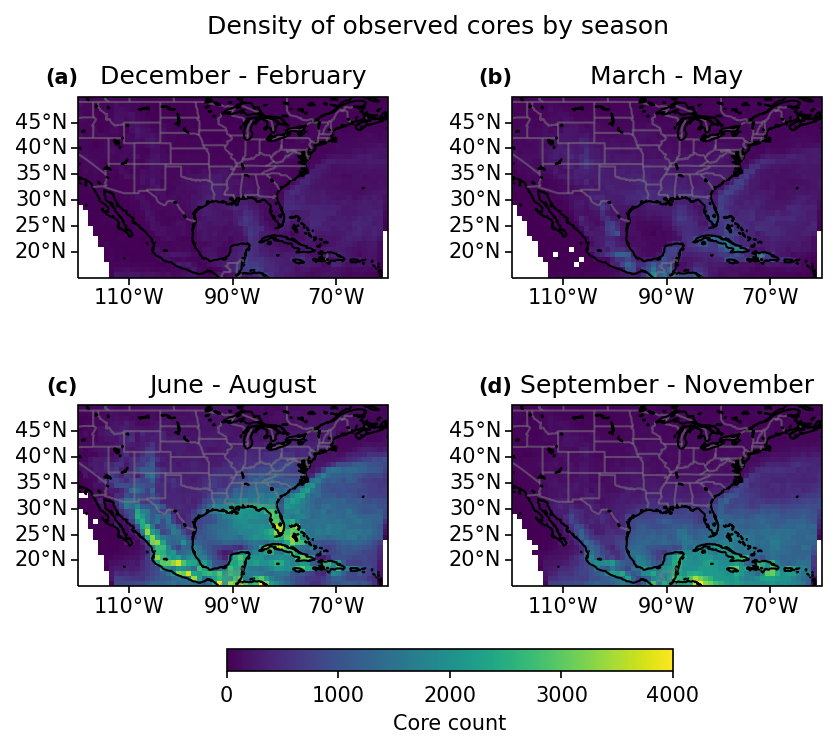
\includegraphics[width=\textwidth]{figures/ch2_03.png}
    \caption{The spatial distribution of observed cores, broken down by season and accumulated into a 1x1 degree grid of latitude and longitude. In winter and spring we see convection mostly over the Rocky Mountains, likely corresponding to winter storms triggered by the orography. In Summer we see the highest frequency of cores, occurring primarily over the Ocean and coastal regions. In Autumn we see increased rates of convection over the Ocean, but not land. }
    \label{fig:core_density_by_season}
\end{figure}

Figure \ref{fig:core_lifetime_map} displays the mean lifetime of observed core over each 1-degree box of latitude and longitude.
Most notably, we see an increase in the average core duration over the Great Plains region.

%f
\begin{figure}[tp]
    \centering
    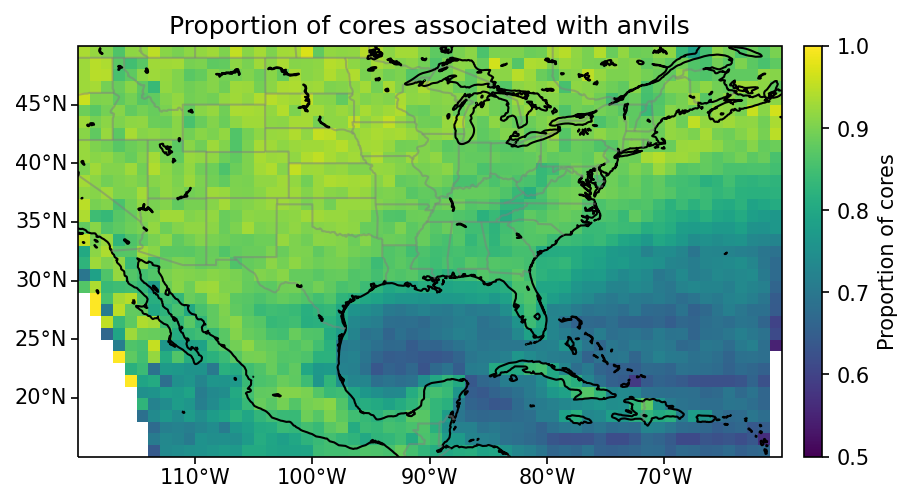
\includegraphics[width=\textwidth]{figures/ch2_04.png}
    \caption{Proportion of cores with anvils}
    \label{fig:cores_with_anvils_map}
\end{figure}

%f
\begin{figure}[tp]
    \centering
    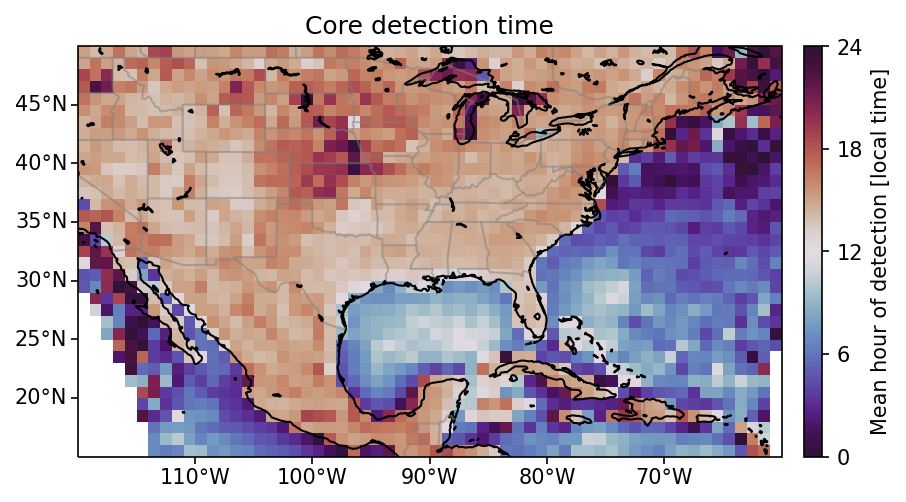
\includegraphics[width=\textwidth]{figures/ch2_05.png}
    \caption[
    The mean time of day of initiation of cores observed within each 1 degree grid box
    ]{
    The mean time of day of initiation of cores observed within each 1 degree grid box. Time of initiation is calculated as the local solar time based on longitude, and the mean is calculated as the circular mean to account for the cyclical aspect of the hour of day.
    }
    \label{fig:core_detection_time_map}
\end{figure}

%f
\begin{figure}[tp]
    \centering
    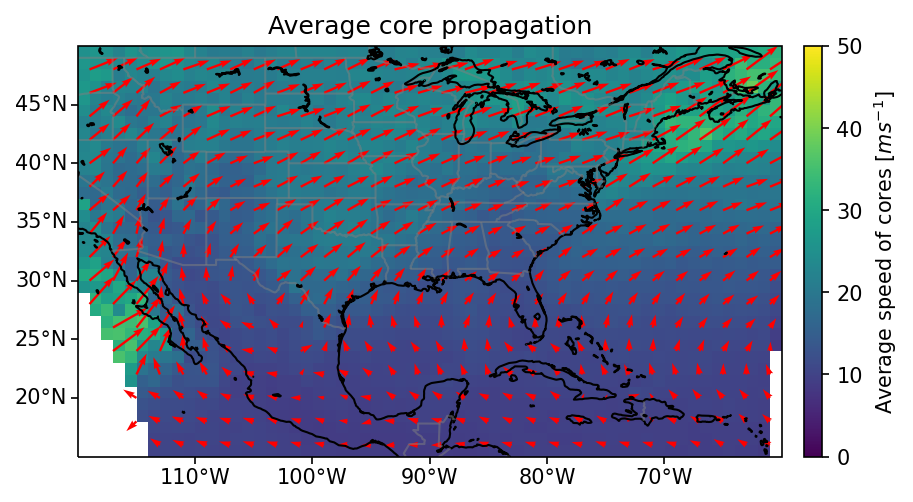
\includegraphics[width=\textwidth]{figures/ch2_06.png}
    \caption{Core propagation direction}
    \label{fig:core_propagation_map}
\end{figure}

%f
\begin{figure}[tp]
    \centering
    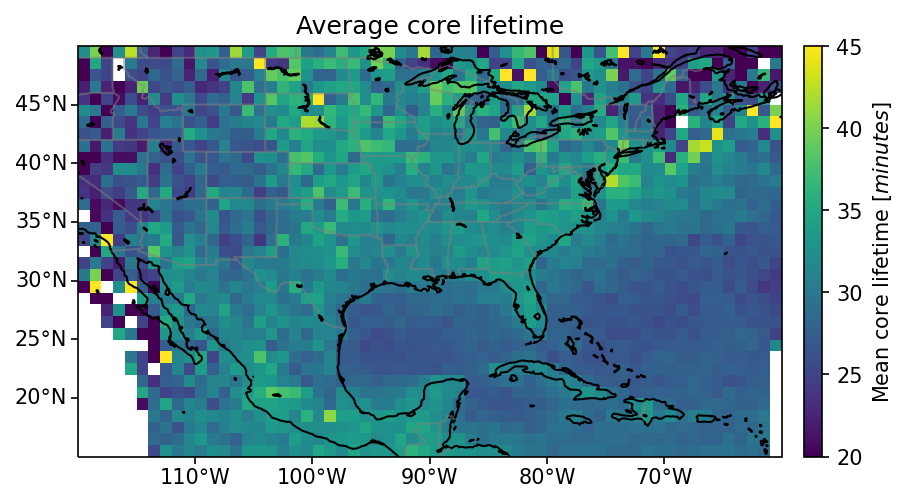
\includegraphics[width=\textwidth]{figures/ch2_07.png}
    \caption{The mean lifetime in minutes of cores within each 1 degree grid box. Increased lifetime is seen over the Great Plains region, corresponding to the more intense convection observed there.}
    \label{fig:core_lifetime_map}
\end{figure}

%f
\begin{figure}[tp]
    \centering
    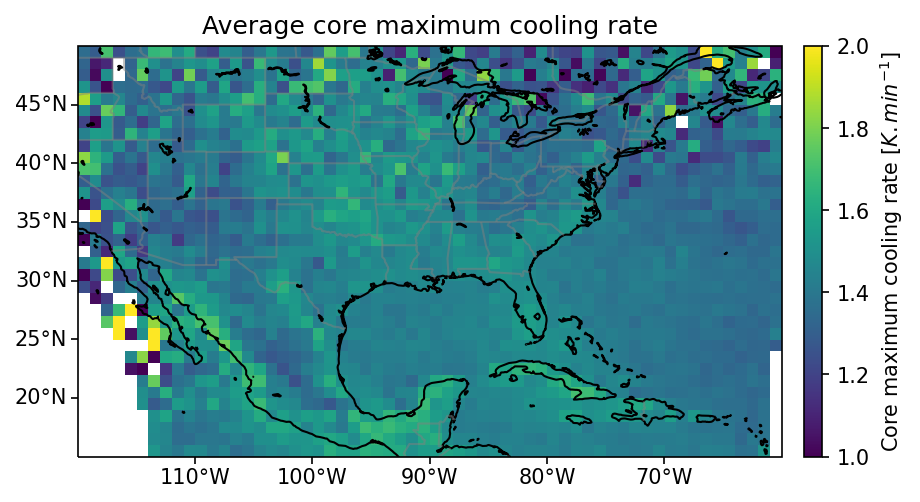
\includegraphics[width=\textwidth]{figures/ch2_08.png}
    \caption{Core maximum cooling rate}
    \label{fig:core_cooling_rate_map}
\end{figure}

%f
\begin{figure}[tp]
    \centering
    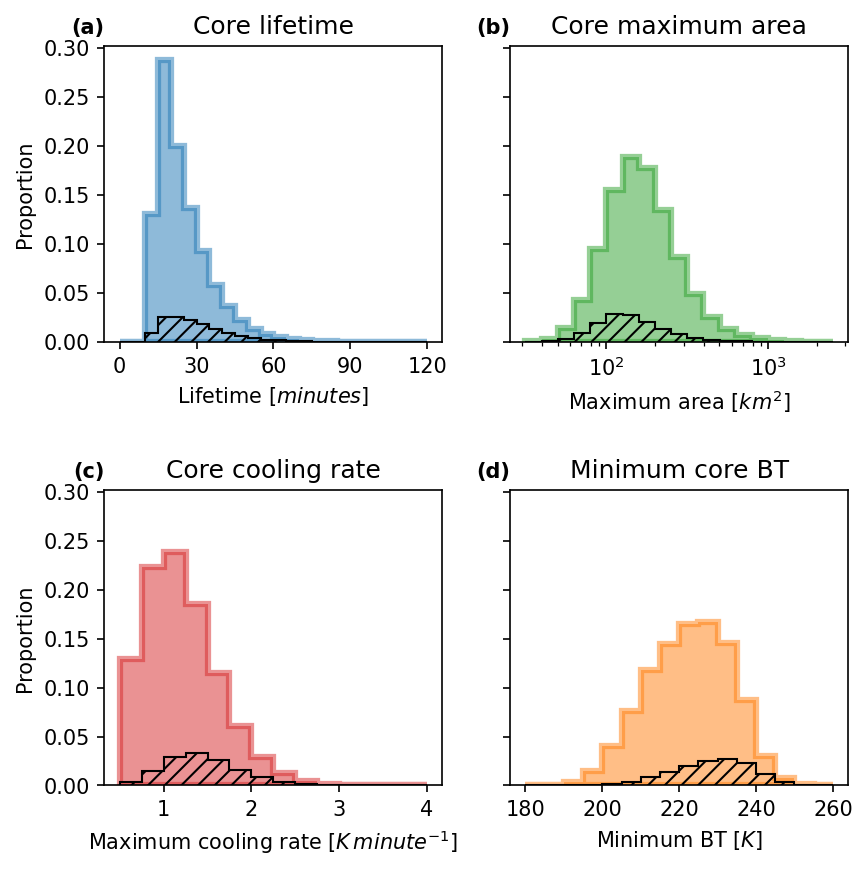
\includegraphics[width=\textwidth]{figures/ch2_09.png}
    \caption{Core properties}
    \label{fig:core_properties}
\end{figure}

%f
\begin{figure}[tp]
    \centering
    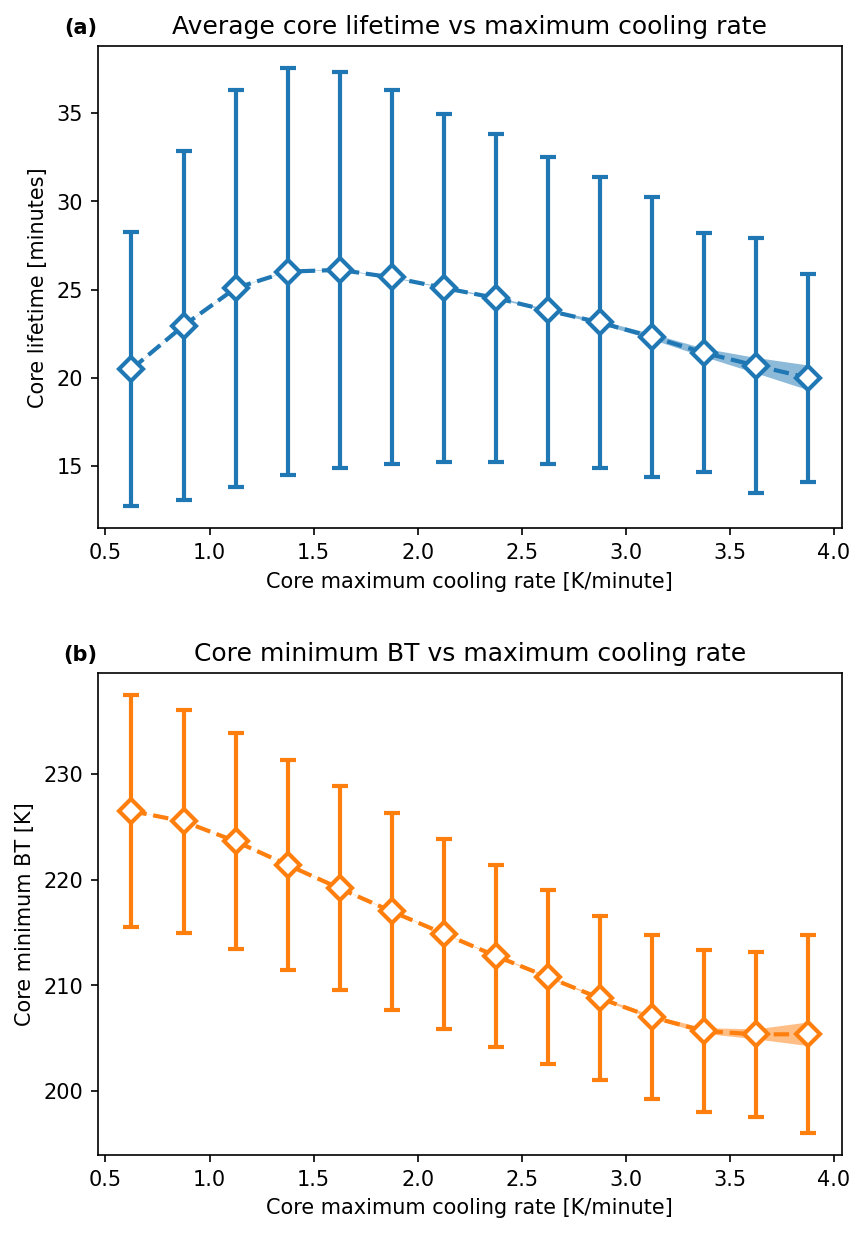
\includegraphics[width=\textwidth]{figures/ch2_10.png}
    \caption{Core cooling rate relations}
    \label{fig:core_cooling_rate_relations}
\end{figure}


%f
\begin{figure}[tp]
    \centering
    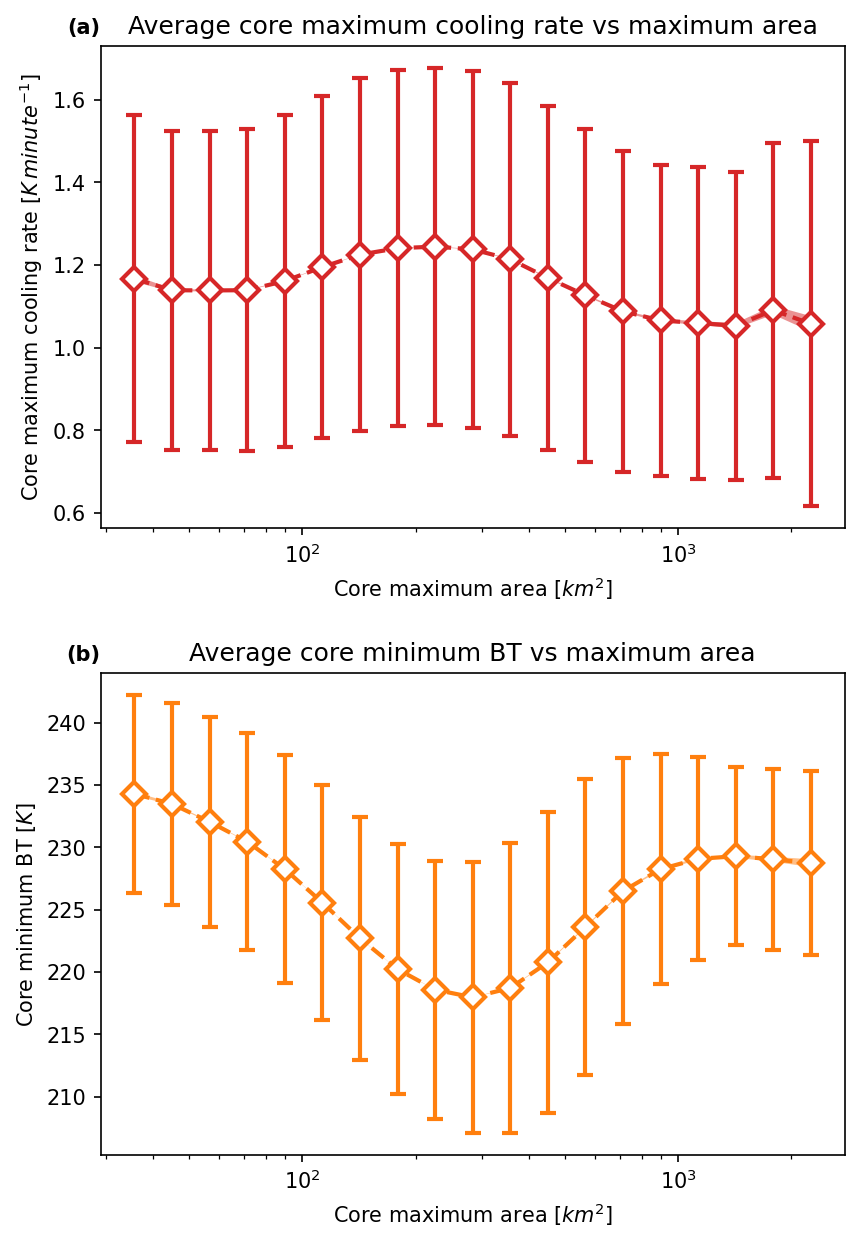
\includegraphics[width=\textwidth]{figures/ch2_11.png}
    \caption{Core area relations}
    \label{fig:core_area_relations}
\end{figure}

In fig. \ref{fig:core_detection_time_map}, we show the mean time of detection for cores detected within each 1-degree lat/lon grid square.
The most notable feature in fig. \ref{fig:core_detection_time_map} is the strong land-sea contrast shown between the Gulf of Mexico and adjacent coastal regions.
Over the Gulf of Mexico, we observe convection to typically occur in the morning, whereas over land we observe most cores in the afternoon.
Over land convective initiation typically occurs due to surface heating from solar radiation, and therefore during the daytime.
In contrast, convective initiation over the ocean is more often due to longwave cooling of the upper atmosphere which is greater at night due to a lack of shortwave heating.
In addition, we see a few major features of detected time of initiation across both land and sea regions.

% %f
% \begin{figure}[tp]
%     \centering
%     \includegraphics[width=\textwidth]{core_detection_time_map.png}
%     \caption{The mean time of day of initiation of cores observed within each 1 degree grid box. Time of initiation is calculated as the local solar time based on longitude, and the mean is calculated as the circular mean to account for the cyclical aspect of the hour of day.}
%     \label{fig:core_detection_time_map}
% \end{figure}

Over the land, we see a later time of initiation over the Northern Great Plains.
Greater CIN in this region leads to a greater requirement for surface heating before convective initiation.
The larger barrier to initiation presented by the increased CIN also leads to greater convective available potential energy (CAPE) production prior to initiation, and hence more vigorous convection, which agrees with the findings in fig. \ref{fig:core_lifetime_map}.

In coastal regions, we also see a change in the time of initiation near to the sea, likely due to sea breeze triggering of convection.
In fig. \ref{fig:sea_breeze_effect} we explicitly show this relationship by plotting the mean time of core detection against distance from the coast.
We see a clear trend towards an earlier time of detection as the distance to the coast reduces, indicative of a sea breeze effect.
The maximum extent of the sea breeze effect extends to between approximately 200\,\unit{km}, similar to the extent of the sea breeze effect quantified using models over the Congo \citep{park_environmental_2020}.

% %f
% \begin{figure}[tp]
%     \centering
%     \includegraphics[width=\textwidth]{sea_breeze_effect.png}
%     \caption{The mean time of detection for observed cores, binned into 25~km intervals of the distance between the location of core initiation and the nearest coastline. A clear trend towards an earlier time of initiation closer to the coast can be seen, with the time of initiation increasing up to approximately 200~km from the nearest coastline.}
%     \label{fig:sea_breeze_effect}
% \end{figure}

To further investigate the differences in observed core properties across North America, we classify observed cores into four regions shown in fig. \ref{fig:regions}.
These four regions were selected due to the observed behaviours of cores seen in previous figures.
The ocean region contains all cores detected over the Gulf of Mexico, the Caribbean and the Western Atlantic.
The coastal region is defined as the areas within 250~km of the ocean region, chosen to investigate the sea-breeze affected areas demonstrated by fig. \ref{fig:sea_breeze_effect}.
The inland areas are further divided into two regions.
Firstly, the Great Plains, to investigate the areas with increased anvil lifetime and later time of detection as seen in figures \ref{fig:core_lifetime_map} and \ref{fig:core_detection_time_map} respectively.
Secondly, the Midwest, in contrast to the Great Plains region, represents more typical over-land convection seen in the dataset.

% %f
% \begin{figure}[tp]
%     \centering
%     \includegraphics[width=\textwidth]{regions_classification.png}
%     \caption{Observations are classified into four regions for further analysis, based on the differences observed in previous figures. Note that the same colours will be used to refer to each region in all subsequent figures. The black dashed line shows the Western limit of observations for the dataset, with no observations recorded further West than this.}
%     \label{fig:regions}
% \end{figure}

% %f
% \begin{figure}[tp]
%     \centering
%     \includegraphics[width=\textwidth]{regions_initiation_dist.png}
%     \caption{Histograms of core time of detection frequency for each of the four regions in fig. \ref{fig:regional_tod}. Core time of initiation is binned into hour intervals.}
%     \label{fig:regional_tod}
% \end{figure}

Figure \ref{fig:regional_tod} shows the distributions of time of day of detection for cores observed within each of the regions shown in fig. \ref{fig:regions}.
The distributions of initiation time for cores over the ocean show a noticeably different distribution to those over land.
The diurnal variation over the ocean is much weaker, however there is still a peak in the morning (and a corresponding low point in the evening) as seen by the average time of initiation in fig. \ref{fig:regional_tod}, which is again explained due to convective initiation being triggered by night-time cooling of the upper atmosphere through longwave emissions.

Over land, we see the highest frequency of cores detected in the coastal region, agreeing with the distributions shown in fig. \ref{fig:core_density_by_season}.
In addition, we see an earlier maximum in the diurnal cycle of 13:00-14:00, compared to that of the Midwest and Great Plains regions of 14:00-15:00.
This agrees with the impact of the sea breeze shown in fig. \ref{fig:sea_breeze_effect}.

Comparing the diurnal cycle of core detection between the Midwest and Great Plains region, we see that the Great Plains region shows a greater frequency of detected cores outside of the peak time period in the afternoon.
In particular, we see increased rates of core detection in the early evening compared to the Midwest region, which is possibly indicative of the bimodal diurnal cycle of deep convection seen previously over the northern great plains \citep{feng_spatiotemporal_2019, li_high-resolution_2021}.

% %f
% \begin{figure}[tp]
%     \centering
%     \includegraphics[width=\textwidth]{regions_lifetime_dist.png}
%     \caption{The frequency distributions of observed core lifetimes for each region, binned by 5 minute intervals.}
%     \label{fig:region_core_lifetimes}
% \end{figure}

% %f
% \begin{figure}[tp]
%     \centering
%     \includegraphics[width=\textwidth]{regions_cooling_rate_dist.png}
%     \caption{The frequency distributions of the maximum cooling rate detected within each core -- which corresponds to the growth rate of the core -- for each region. Binned by 0.1~K/minute intervals.}
%     \label{fig:region_cooling_rate}
% \end{figure}

In fig. \ref{fig:region_core_lifetimes} and fig. \ref{fig:region_cooling_rate} we see the distributions of core lifetime and maximum core cooling rate respectively for each of the regions.
The distribution of core lifetimes shows little difference between each region, with the Great Plains having a marginally longer tail.
The distribution of core cooling rates again shows little difference between each region, however there is a more noticeable increase in the frequency of higher cooling rates over the Great Plains, indicative of more intense convection in the region.


% \section{Observed trends in core behaviour}



% %f
% \begin{figure}[tp]
%     \centering
%     \includegraphics[width=\textwidth]{core_lifetime_vs_tod.png}
%     \caption{}
%     % \label{fig:detected_anvils}
% \end{figure}


% %f
% \begin{figure}[tp]
%     \centering
%     \includegraphics[width=\textwidth]{core_lifetime_vs_cooling_rate.png}
%     \caption{The mean core lifetime for each region, grouped by the maximum core cooling rate in 0.1~K/minute intervals.}
%     \label{fig:lifetime_vs_tod}
% \end{figure}

Figure \ref{fig:lifetime_vs_tod} compares how the average lifetime of detected cores changes with their maximum observed cooling rate.
For low values of core cooling rate, we see a similar, positive linear relationship between cooling rate and lifetime between all regions, indicating that more intense convection leads to longer periods of cores being observed.
However, for values beyond cooling rates of 1.0-1.2\,\unit{K minute\textsuperscript{-1}} we see an inflection in the relationship, with larger cooling rates leading to shorter lifetimes.
This may be explained by the influence of the tropopause on the detection period of growing convection.
For convective cores that reach the tropopause, this sets a hard limit on the maximum period over which convective growth is detected by cloud-top cooling.
As a result, deep convective cores which display larger cloud-top cooling rates will reach the tropopause faster and hence have a shorter detected lifetime.
However, the reduced number of observations for cores with large cooling rates (>1\,\unit{K minute\textsuperscript{-1}}) means that these values should be treated with caution as they may be a result of uncertainty.

% %f
% \begin{figure}[tp]
%     \centering
%     \includegraphics[width=\textwidth]{phase_development.png}
%     \caption{}
%     % \label{fig:detected_anvils}
% \end{figure}

% %f
% \begin{figure}[tp]
%     \centering
%     \includegraphics[width=\textwidth]{phase_vs_temperature.png}
%     \caption{}
%     % \label{fig:detected_anvils}
% \end{figure}

\subsection{Distributions and properties of observed anvil clouds}

By tracking the anvils associated with detected cores, we can investigate the differences in the properties of anvil clouds in response to changes in the cores.
Figure \ref{fig:multicore_frequency} show the frequency of anvil clouds detected with different numbers of cores.
We observe that the majority of anvils form from a single core, with a continuous decay in the number of anvils observed with an increasing number of cores.
It should be noted however, that as we are detecting cores through observing regions of cooling cloud top temperatures, it is harder to detect cores within mature anvils and as a result we may underestimate the number of cores in larger systems.

%f
\begin{figure}[tp]
    \centering
    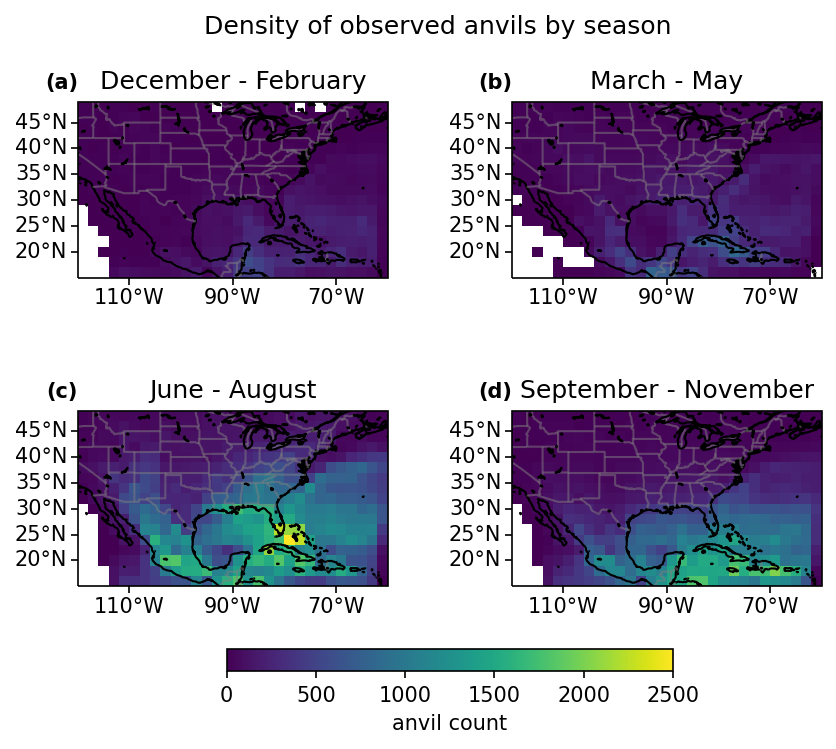
\includegraphics[width=\textwidth]{figures/ch2_12.png}
    \caption{Spatial distribution of observed anvils by season, binned to 2x2 degree grid.}
    \label{fig:anvil_distribution_map}
\end{figure}

%f
\begin{figure}[tp]
    \centering
    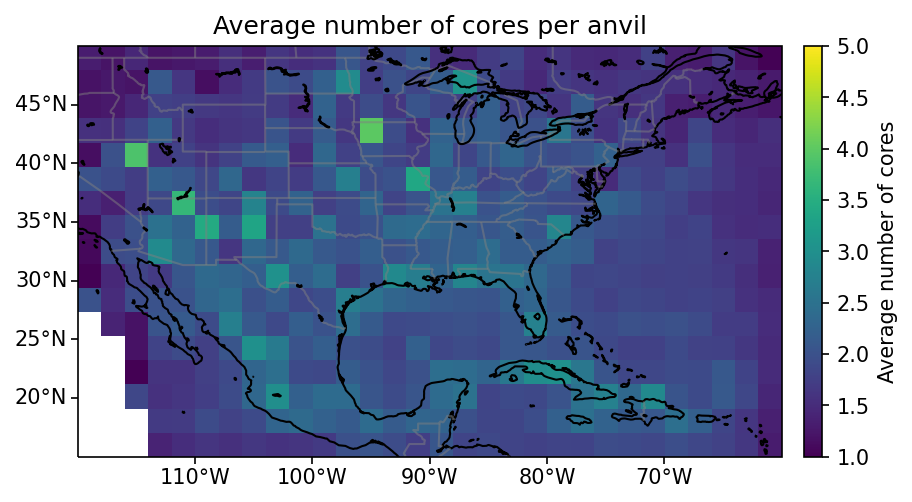
\includegraphics[width=\textwidth]{figures/ch2_13.png}
    \caption{Average number of cores per anvil}
    \label{fig:anvil_number_of_cores_map}
\end{figure}

%f
\begin{figure}[tp]
    \centering
    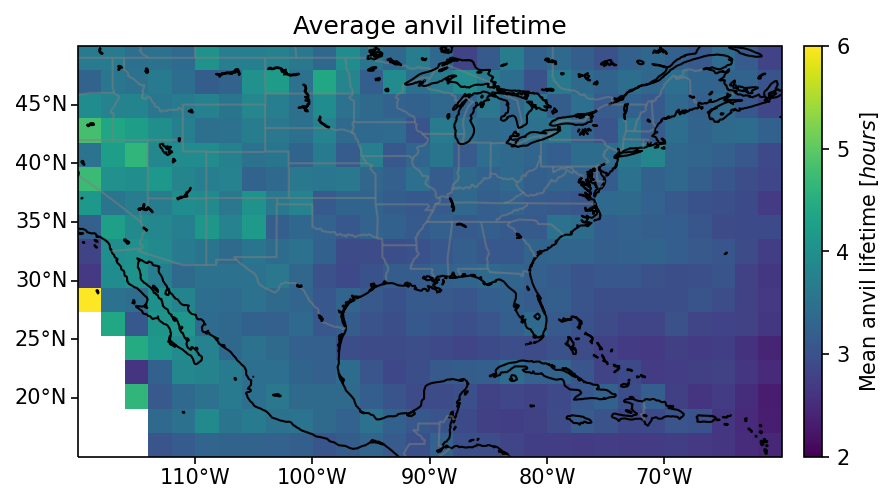
\includegraphics[width=\textwidth]{figures/ch2_14.png}
    \caption{Average anvil lifetime}
    \label{fig:anvil_lifetime_map}
\end{figure}

%f
\begin{figure}[tp]
    \centering
    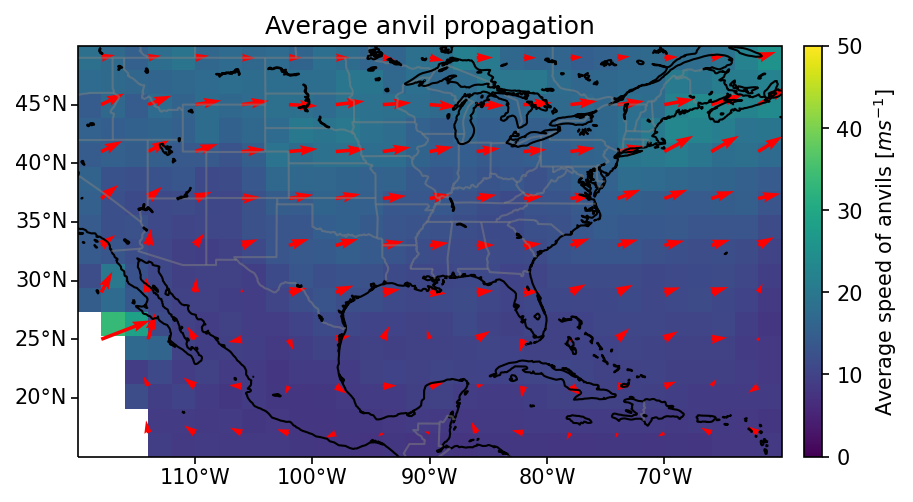
\includegraphics[width=\textwidth]{figures/ch2_15.png}
    \caption{Anvil propagation}
    \label{fig:anvil_propagation_map}
\end{figure}

%f
\begin{figure}[tp]
    \centering
    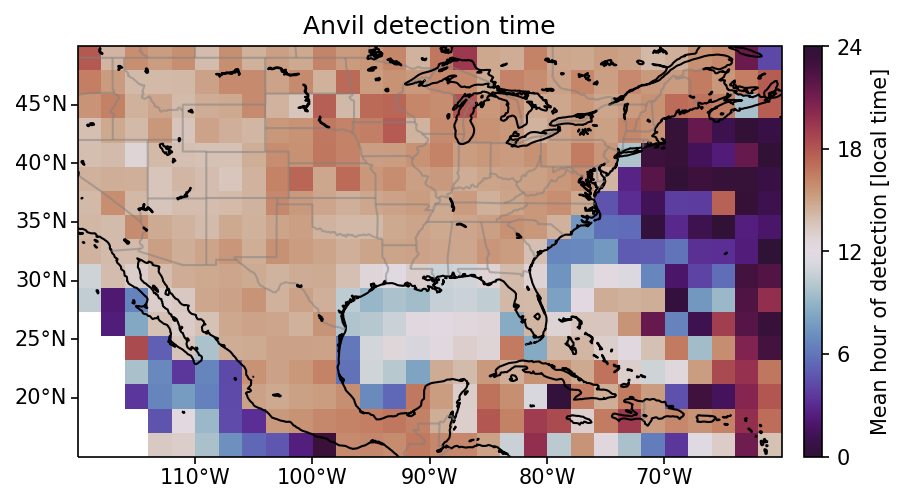
\includegraphics[width=\textwidth]{figures/ch2_16.png}
    \caption{Anvil time of detection}
    \label{fig:anvil_detection_time_map}
\end{figure}

%f
\begin{figure}[tp]
    \centering
    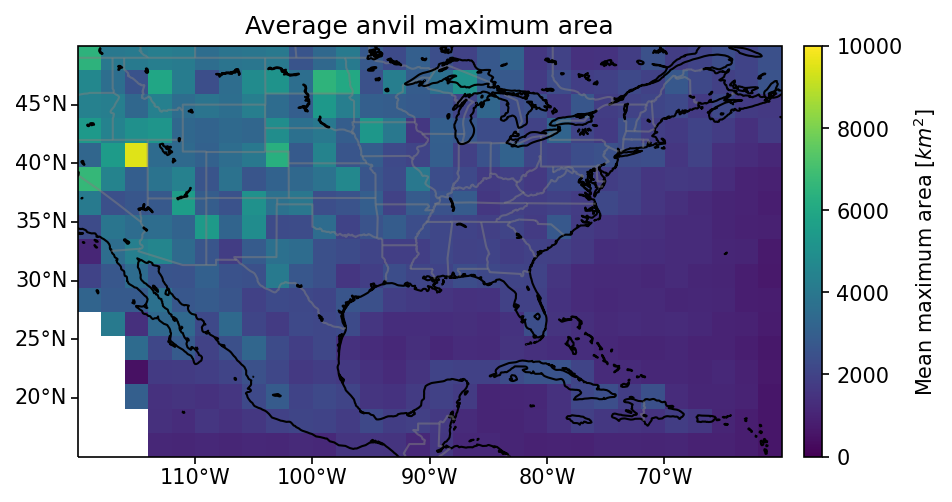
\includegraphics[width=\textwidth]{figures/ch2_17.png}
    \caption{Anvil maximum area}
    \label{fig:anvil_area_map}
\end{figure}

%f
\begin{figure}[tp]
    \centering
    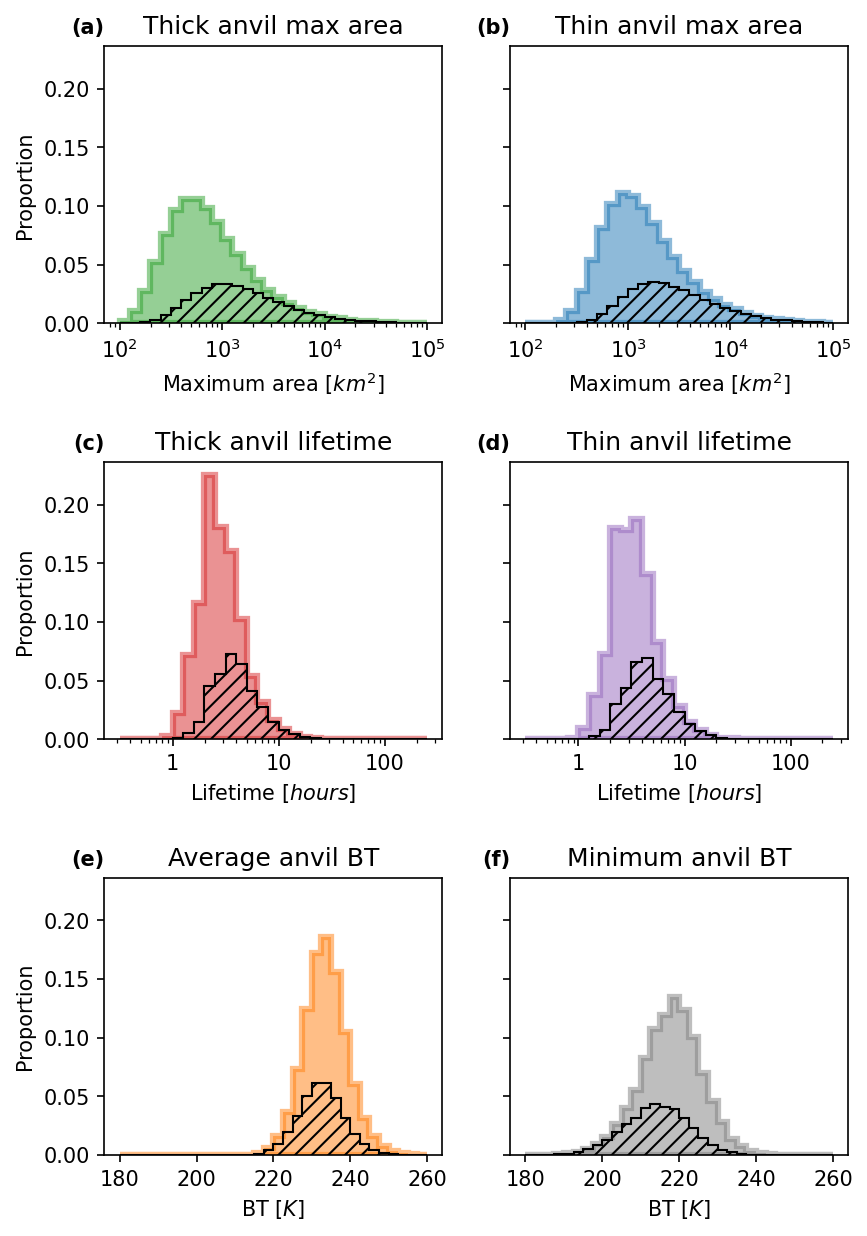
\includegraphics[width=\textwidth]{figures/ch2_18.png}
    \caption{Anvil properties}
    \label{fig:anvil_properties}
\end{figure}

%f
\begin{figure}[tp]
    \centering
    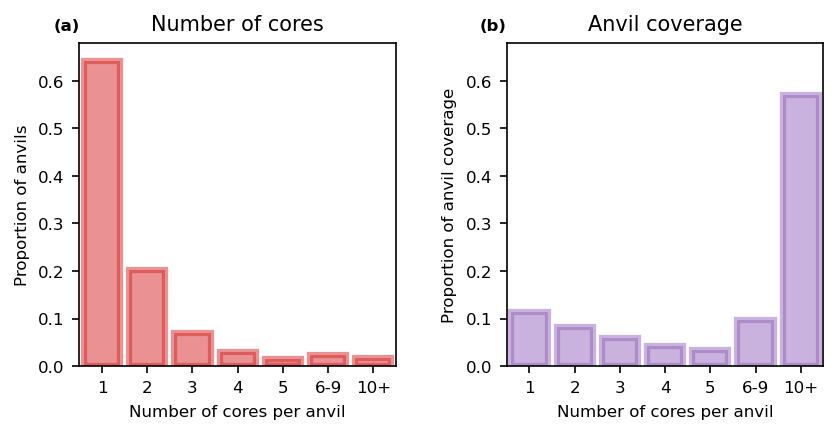
\includegraphics[width=\textwidth]{figures/ch2_19.png}
    \caption{Anvil number of core distribution and coverage}
    \label{fig:anvil_cores_and_coverage}
\end{figure}

%f
\begin{figure}[tp]
    \centering
    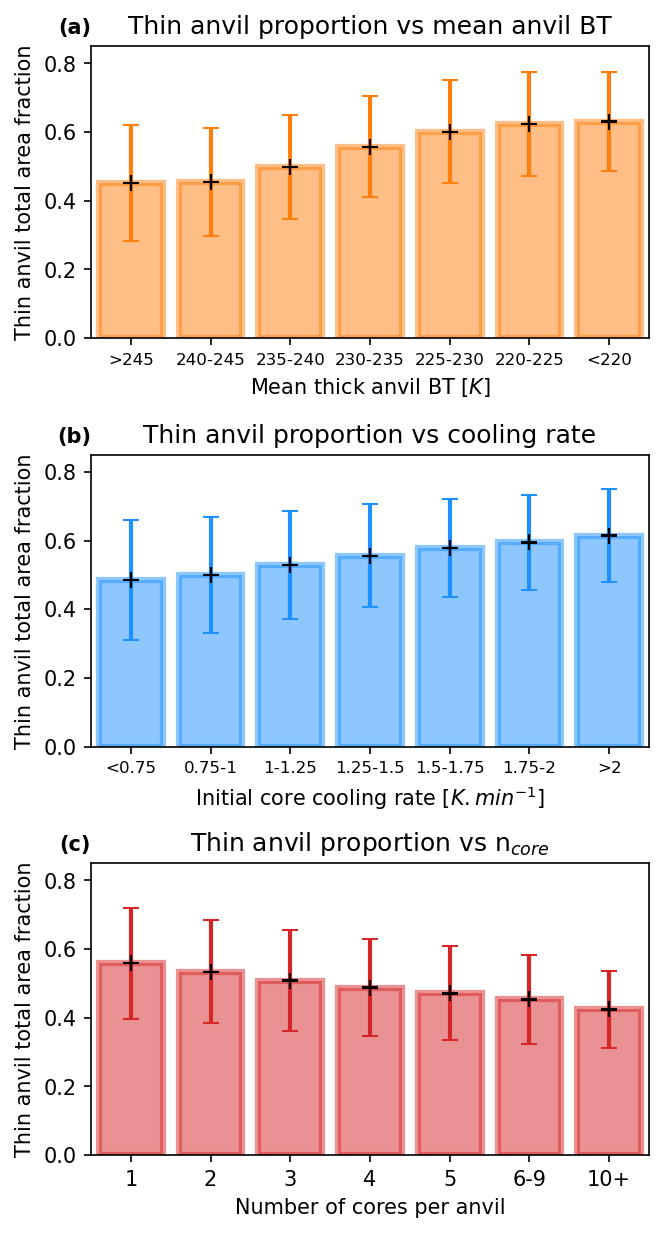
\includegraphics[width=0.75\textwidth]{figures/ch2_20.png}
    \caption{Thin anvil proportion}
    \label{fig:thin_anvil_proportion}
\end{figure}

%f
\begin{figure}[tp]
    \centering
    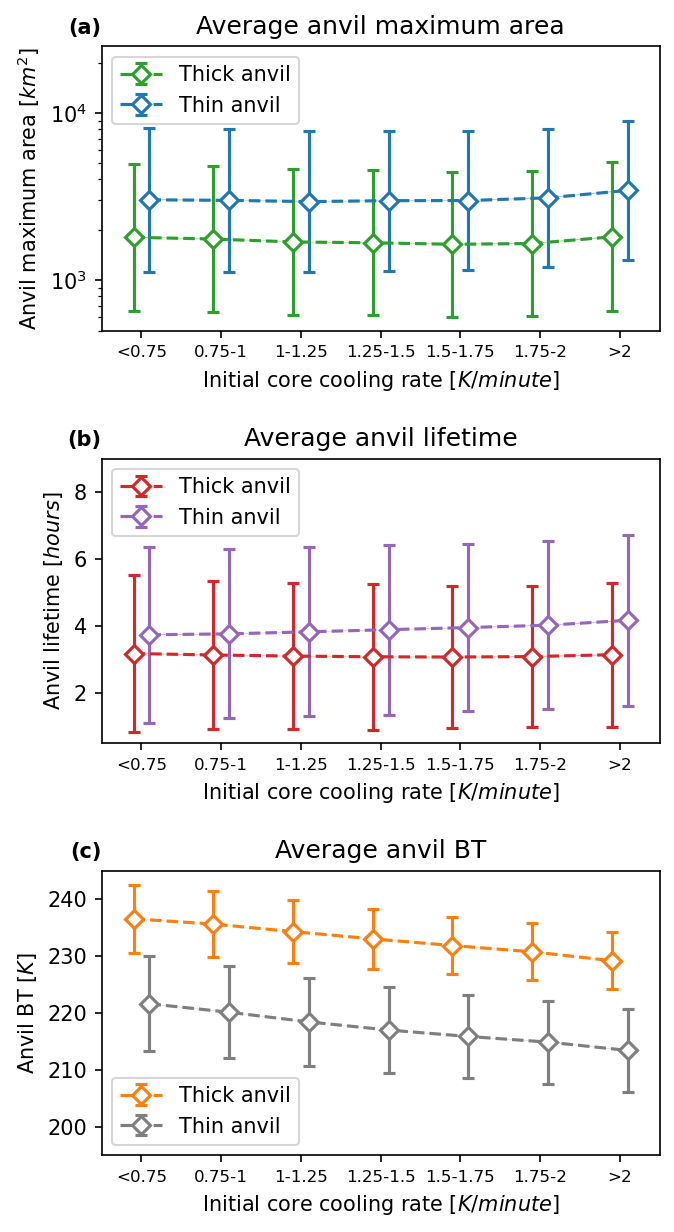
\includegraphics[width=0.75\textwidth]{figures/ch2_21.png}
    \caption{Anvil properties by initial cooling rate}
    \label{fig:anvil_cooling_rate_propeties}
\end{figure}

%f
\begin{figure}[tp]
    \centering
    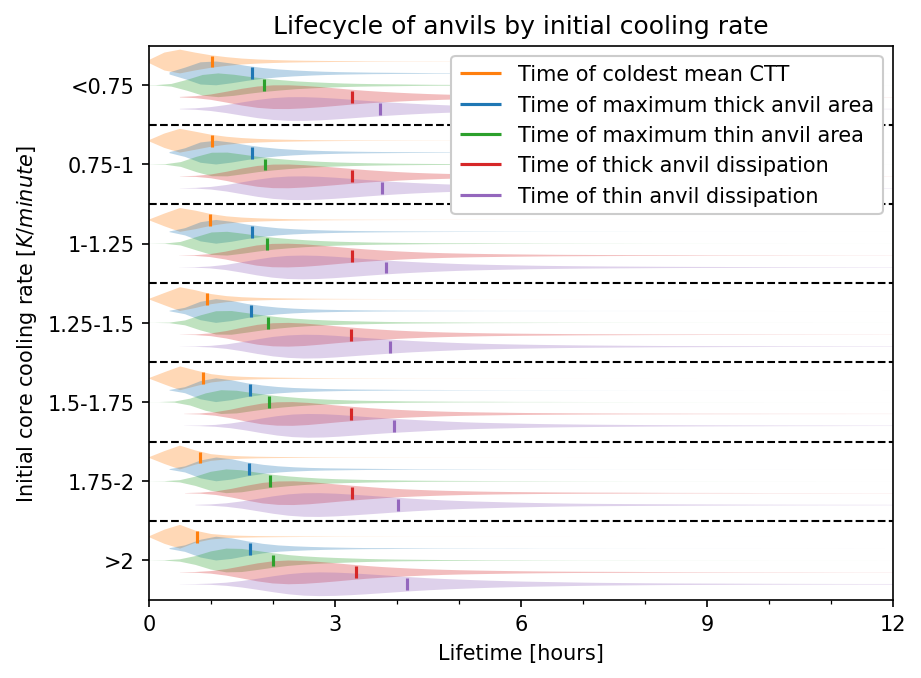
\includegraphics[width=\textwidth]{figures/ch2_22.png}
    \caption{Anvil lifecycle by initial cooling rate}
    \label{fig:anvil_cooling_rate_lifecycle}
\end{figure}

%f
\begin{figure}[tp]
    \centering
    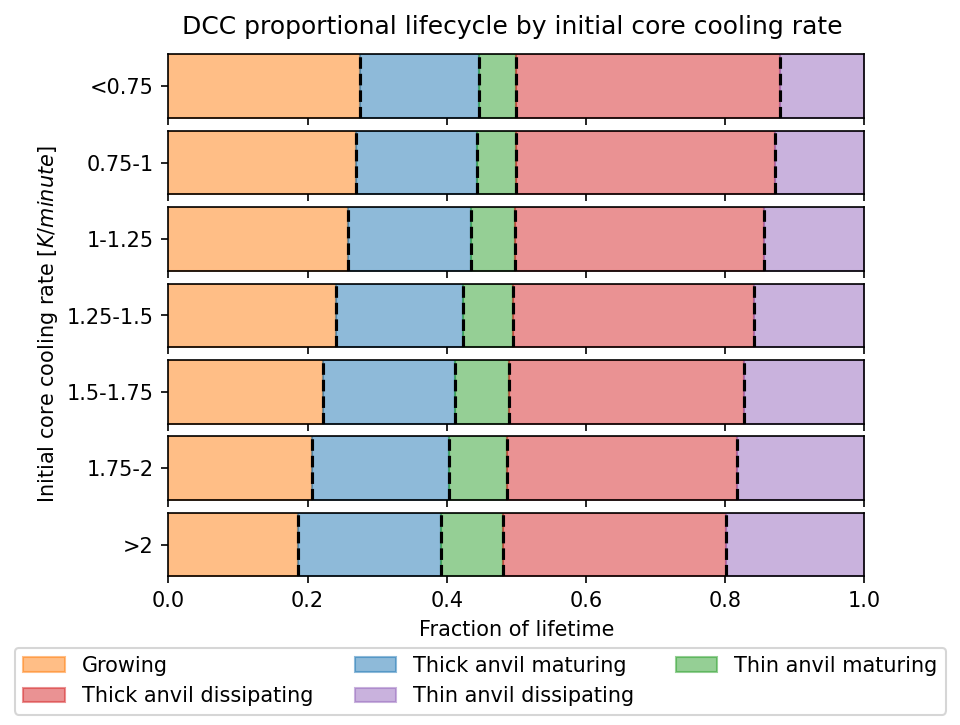
\includegraphics[width=\textwidth]{figures/ch2_23.png}
    \caption{Anvil proportional lifecycle by initial cooling rate}
    \label{fig:anvil_cooling_rate_proportional_lifecycle}
\end{figure}

%f
\begin{figure}[tp]
    \centering
    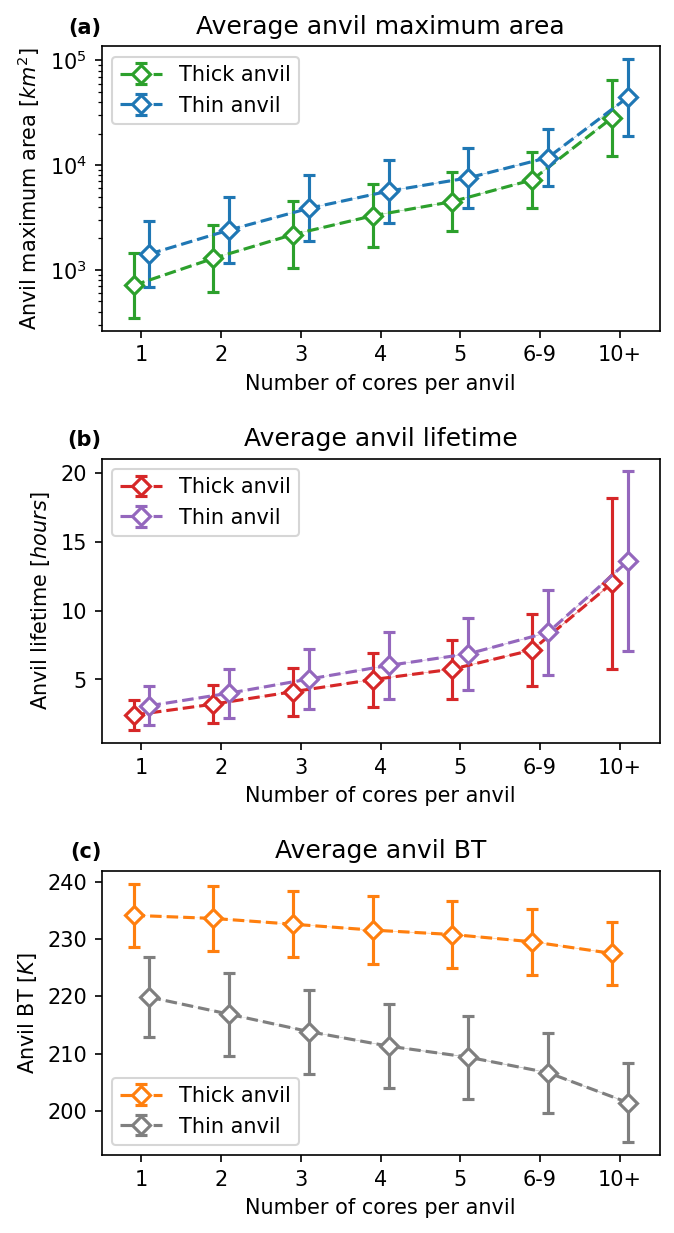
\includegraphics[width=0.75\textwidth]{figures/ch2_24.png}
    \caption{Anvil properties by number of cores}
    \label{fig:anvil_number_of_cores_propeties}
\end{figure}

%f
\begin{figure}[tp]
    \centering
    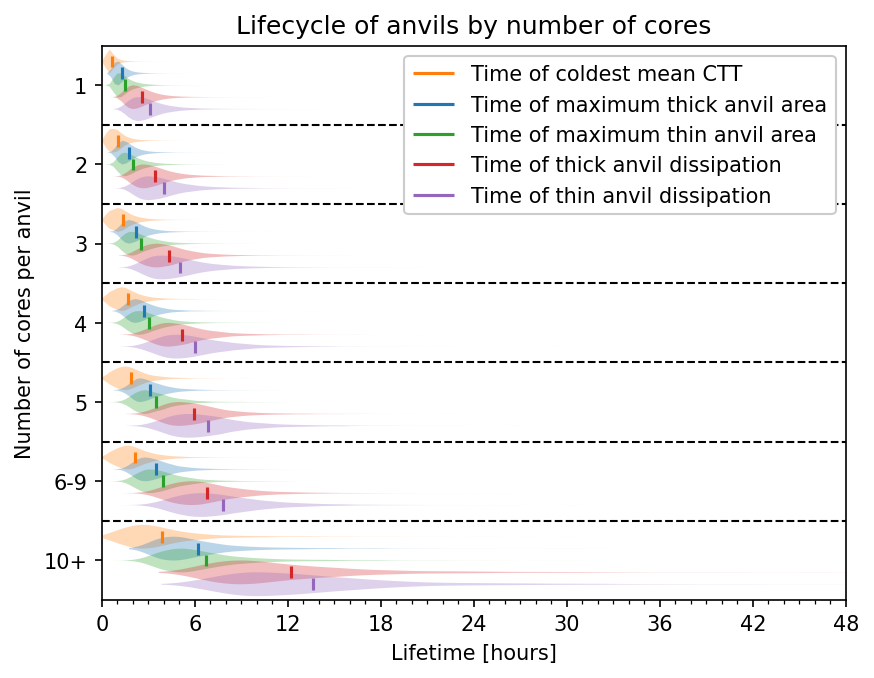
\includegraphics[width=\textwidth]{figures/ch2_25.png}
    \caption{Anvil lifecycle by number of cores}
    \label{fig:anvil_number_of_cores_lifecycle}
\end{figure}

%f
\begin{figure}[tp]
    \centering
    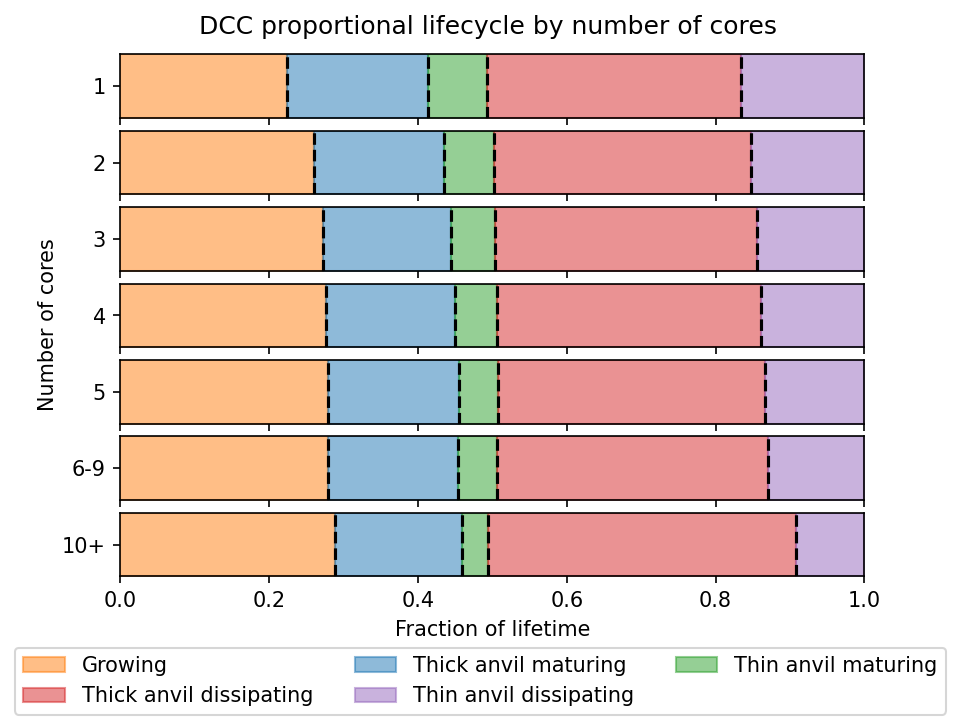
\includegraphics[width=\textwidth]{figures/ch2_26.png}
    \caption{Anvil proportional lifecycle by number of cores}
    \label{fig:anvil_number_of_cores_proportional_lifecycle}
\end{figure}

% %f
% \begin{figure}[tp]
%     \centering
%     \includegraphics[width=\textwidth]{cores_per_anvil_all.png}
%     \caption{Histogram of the frequency of anvils observed by number of cores.}
%     \label{fig:multicore_frequency}
% \end{figure}

Figure \ref{fig:multicore_fraction_map} shows the fraction of anvils detected that are associated with more than one core in each 1x1 degree grid square.
There is a noticeable increase in the fraction of multi-core anvils with increasing latitude.
This is possibly due to the greater influence of large-scale forcing such as the jet stream as we move further from the tropics.

% %f
% \begin{figure}[tp]
%     \centering
%     \includegraphics[width=\textwidth]{multicore_anvil_density.png}
%     \caption{The fraction of anvils observed within each 1x1 degree box that are associated with multiple cores.}
%     \label{fig:multicore_fraction_map}
% \end{figure}

Figures \ref{fig:anvil_lifetime_by_core} and \ref{fig:thin_anvil_lifetime_by_core} show how the average lifetime of observed anvil clouds varies depending on the number of cores associated with each anvil.
In both cases, we observe the lifetime of the anvil to increase with the number of cores.
In general, anvils observed over land have longer lifetimes than those over the coast and ocean.

% %f
% \begin{figure}[tp]
%     \centering
%     \includegraphics[width=\textwidth]{thick_anvil_lifetime_cores.png}
%     \caption{The mean lifetime of observed thick anvil clouds against the number of cores associated with the anvil cloud.}
%     \label{fig:anvil_lifetime_by_core}
% \end{figure}

Of particular note in fig. \ref{fig:anvil_lifetime_by_core} is the Great Plains region.
Single-core anvils in this region have short lifetimes similar to those of anvils over the ocean and coast.
However, the lifetime of anvils over the Great Plains increases more rapidly with the number of cores compared to other regions, and it displays longer lifetimes for multi-core anvils than other regions, potentially indicating greater dynamical interactions.
In fig. \ref{fig:thin_anvil_lifetime_by_core}, however, we observe that in the Great Plains region the lifetime of the thin anvil cloud for single-core \acrshort{dcc}s is similar to those in the Midwest.
This indicates that anvils in the Great Plains region have a longer dissipating phase than those of other regions.
It should also be noted that no significant differences in average core lifetime or growth rates are found for the cores observed associates with multi-core and single-core anvils, so these differences in the anvil behaviour are due to the interactions between multiple cores, not the individual differences in the cores.

% %f
% \begin{figure}[tp]
%     \centering
%     \includegraphics[width=\textwidth]{thin_anvil_lifetime_cores.png}
%     \caption{The mean lifetime of observed thin anvil clouds against the number of cores associated with the anvil cloud.}
%     \label{fig:thin_anvil_lifetime_by_core}
% \end{figure}


\section{Conclusions}  %% \conclusions[modified heading if necessary]

By producing the first continental scale dataset of both \acrshort{dcc} cores and anvils, we are able to analyse a large number of detected deep convective systems.
We have been able to show a number of key differences in the seasonal, diurnal and regional patterns of \acrshort{dcc}s across the continental US.
The spatial distribution of \acrshort{dcc} cores across the continental US depends strongly on the seasonal cycle.
The properties of cores themselves, including the lifetime, cooling rate, and time of initiation, have regional dependencies.
We see a large land/sea contrast in time of initiation, and a sea breeze effect which extends for approximately 200\,\unit{km} inland.
In addition, we see differences in the distribution of core time of detection between the two inland regions -- the Midwest and the Great Plains -- with the Great Plains showing a greater spread of convection throughout the night time.
In addition, the Great Plains region shows increased core cooling rates and lifetimes compared to other regions, both of which are associated with more intense convection.
It may be the case that this later time of initiation results in more intense deep convective storms.
The distribution of lifetimes of observed cores shows less difference between different regions, indicating that a number of competing factors may be controlling this property.

While the majority of observed anvil clouds are associated with a single growing core, there remain a large number of multi-core anvils detected in our dataset.
The frequency of multi-core anvils as a proportion of all observed anvils increases with latitude.
Finally, while the properties of the individual growing cores observed in single- and multi-core anvils show no significant difference, the lifetime of anvils clouds shows a large increase with the number of cores.
In addition, the extended lifetime of the thin anvil cloud compared to that of the thick anvil over the Great Plains region may be evidence of the impact of the intensity of convection on the dissipating phase of the \acrshort{dcc}.

Overall, a number of competing factors influence the properties of both \acrshort{dcc} cores and anvils, including the seasonal and diurnal cycles, region, and the number of cores associated with each anvil.
These factors require careful consideration when investigating the response of deep convection to external influences.
Future work will focus on connecting the behaviour of observed \acrshort{dcc}s to meteorological changes including surface temperature, humidity, CAPE and CIN, as well as the impact of aerosols on \acrshort{dcc}s.
Furthermore, we will quantify to radiative impacts of anvil clouds across their lifecycle, and aim to investigate the feedbacks of these radiative effects on subsequent convection.

